\documentclass{article}
%packages
\usepackage{graphicx}
\usepackage[utf8]{inputenc}
\usepackage[T1]{fontenc}
\usepackage[frenchb]{babel}
\usepackage[a4paper]{geometry}

\begin{document}
%title
\begin{titlepage}
  \vspace{-20px}
  \begin{tabular}{l}
    \textsc{Blin} S\'ebastien\\
    \textsc{Collin} Pierre-Henri
  \end{tabular}
  \hfill \vspace{10px}
\includegraphics[scale=0.1]{esir.png}\\
  \vfill
  \begin{center}
    \Huge{\'Ecole sup\'erieure d'ing\'enieurs de Rennes}\\
    \vspace{1cm}
    \LARGE{1\`ere Ann\'ee}\\
    \large{Parcours Informatique}\\
    \vspace{0.5cm}\hrule\vspace{0.5cm}
    \LARGE{\textbf{Algorithmie et complexité}}\\
    \Large{Compte-Rendu TP2}
    \vspace{0.5cm}\hrule
    \vfill
    \vfill
  \end{center}
  \begin{flushleft}
    \Large{Sous l'encadrement de~:}\\
    \vspace{0.2cm}
    \large{{Ridoux} Olivier}\\
    \large{{Maurel} Pierre}
  \end{flushleft}
  \vfill
\end{titlepage}

\section{Objectif}
Ce second TP a pour objectif de nous faire implémenter la transformée de Fourier rapide et de nous faire découvrir 2 de ses applications. Dans la première partie de ce TP, nous allons donc utiliser la transformée de Fourier pour pouvoir réaliser des multiplications de polynômes. Dans la seconde partie, nous allons utiliser la transformée de Fourier pour pouvoir compresser des images, comme le fait en partie la compression jpeg par exemple.
\section{Multiplication de polynômes}
\subsection{Moyens mis en \oe uvre}
Pour la partie implémentation, nous nous sommes basés sur l'algorithme donné pour implémenter la transformée de Fourier. Voici notre méthode combine
\begin{verbatim}
  //"combine" c1 et c2 selon la formule vue en TD
  // c1 et c2 sont de même taille
  // la taille du résultat est le double de la taille de c1
  public static CpxTab combine(CpxTab c1, CpxTab c2) {
    assert (c1.taille()==c2.taille()) : 
    "combine: c1 et c2 ne sont pas de même taille, taille c1="
    +c1.taille()+" taille c2="+c2.taille();
    int taille = c1.taille()+c2.taille();
    CpxTab res = new CpxTab(taille);
    for(int i=0; i<c1.taille(); i++)
    {
      //première partie du tableau
      double termeReel =c2.get_p_reel(i)*Math.cos(2*Math.PI*i/taille)
      -c2.get_p_imag(i)*Math.sin(2*Math.PI*i/taille);
      double termeImag = c2.get_p_imag(i)*Math.cos(2*Math.PI*i/taille)
      +c2.get_p_reel(i)*Math.sin(2*Math.PI*i/taille);
      
      res.set_p_reel(i,c1.get_p_reel(i)+termeReel);
      res.set_p_imag(i,c1.get_p_imag(i)+termeImag);
      //deuxième partie du tableau
      res.set_p_reel(c1.taille()+i,c1.get_p_reel(i)-termeReel);
      res.set_p_imag(c1.taille()+i,c1.get_p_imag(i)-termeImag);
      
    }
    return res;
  }
\end{verbatim}
Et la méthode pour calculer la FFT :
\begin{verbatim}
  //renvoie la TFD d'un tableau de complexes
  //la taille de x doit être une puissance de 2
  public static CpxTab FFT(CpxTab x) {
    //A FAIRE : Test d'arrêt
    if(x.taille()==1)
      return x;
    assert (x.taille()%2==0) : "FFT: la taille de x doit être une puissance de 2";
    
    CpxTab pair = new CpxTab(x.taille()/2);
    CpxTab impair = new CpxTab(x.taille()/2);
    for(int i=0; i<x.taille(); i++)
    {
      if(i%2==0)
      {
        pair.set_p_reel(i/2,x.get_p_reel(i));
        pair.set_p_imag(i/2,x.get_p_imag(i));
      }
      else
      {
        impair.set_p_reel((i-1)/2,x.get_p_reel(i));
        impair.set_p_imag((i-1)/2,x.get_p_imag(i));
      }
    }

    return combine(FFT(pair), FFT(impair));
  }
\end{verbatim}
Enfin la méthode inverse
\begin{verbatim}
  //renvoie la tr\tansformée de Fourier inverse de y
  public static CpxTab FFT_inverse(CpxTab y) {
    //A FAIRE
    CpxTab t = new CpxTab(y.taille());
    for(int i = 0; i < y.taille(); ++i)
      t.set_p_reel(i, 1./(double)y.taille());
    return CpxTab.multiplie(t, (FFT(y.conjuge())).conjuge());
  }
\end{verbatim}
Nous l'avons ensuite testé sur des polynômes pour comparer les méthodes avec transformée de Fourier rapide et la méthode classique.
\subsection{Résultats}

\begin{figure}
	\begin{center}
		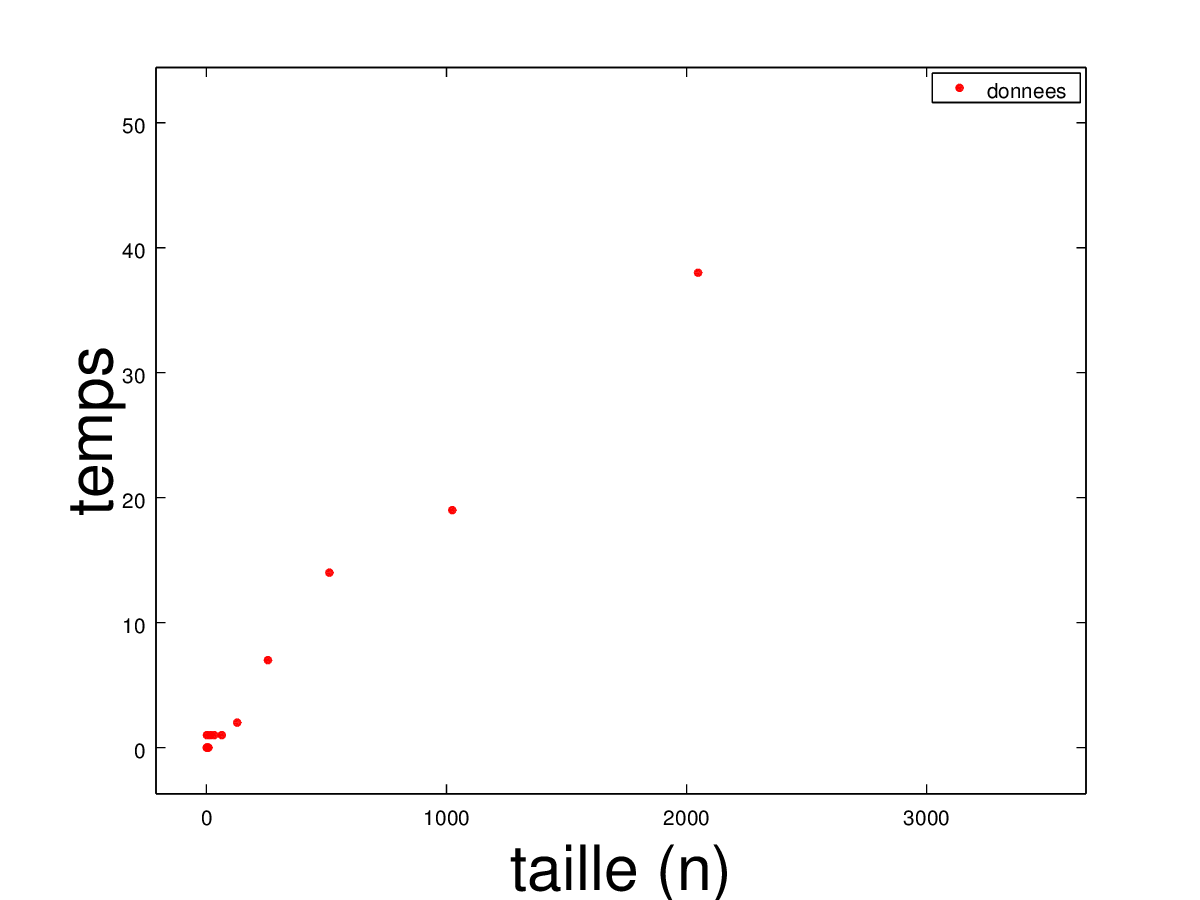
\includegraphics[scale=0.5]{FFTSmall}\\
		Avec FFT
	\end{center}
\end{figure}
\begin{figure}
	\begin{center}
		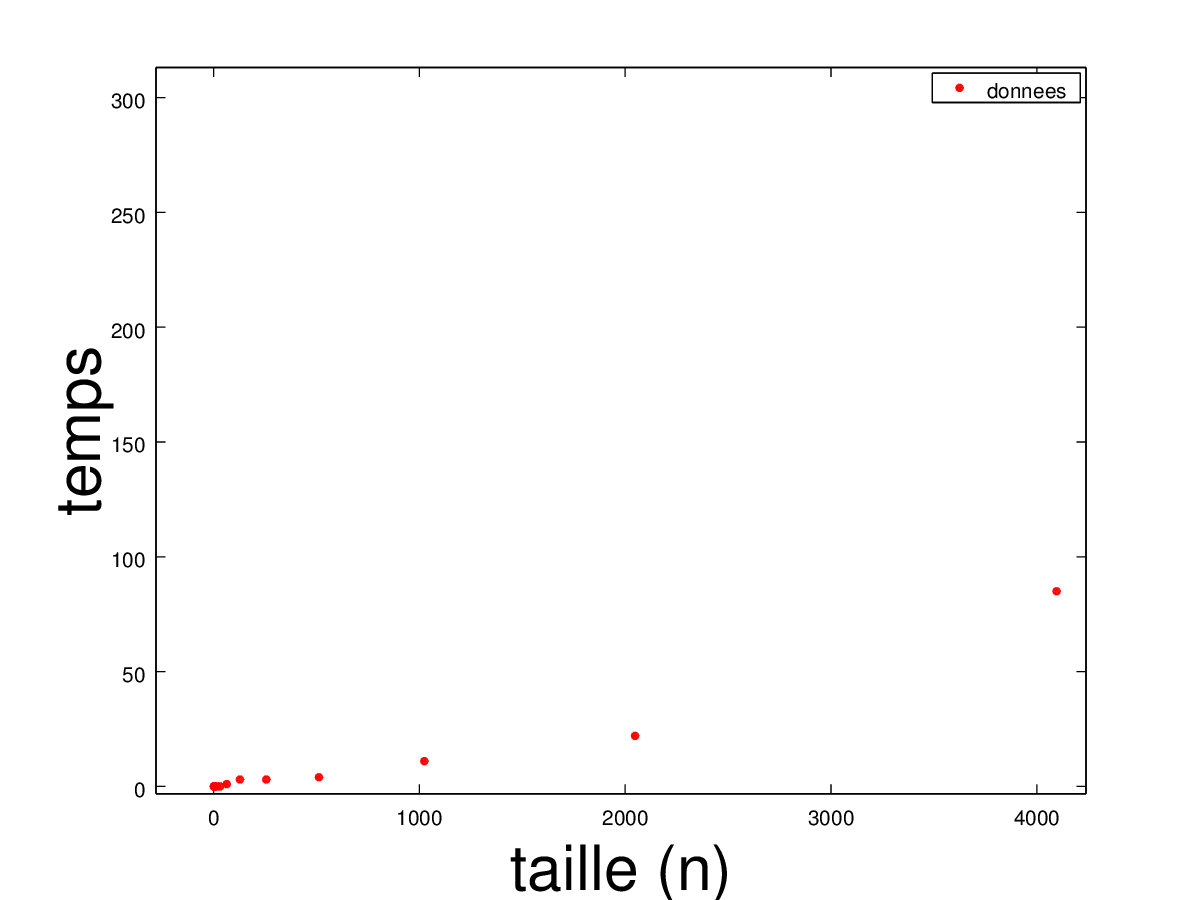
\includegraphics[scale=0.5]{NoFFTSmall}\\
		Sans FFT
	\end{center}
\end{figure}
On remarque que la méthode avec transformée de Fourier est plus rapide pour un polynôme a 4000 coefficients. En dessous, les méthodes sont à peu prêt équivalentes au niveau du temps.

\section{Compression d'images}
\subsection{Moyens mis en \oe uvre}
Dans la seconde partie de ce TP nous avons tout d'abord calculé la TFD de différents signaux (constant, sinusoides, etc.). Nous avons alors remarqué que la TFD nous donne la fréquence. Par exemple pour un signal constant, le tableau de sortie nous donne seulement la première valeur ($[16.0,0,0,0,0,0,0,0,0,0,0,0,0,0,0,0]$). Pour une sinusoide, on obtient 2 valeurs par symétrique ($[0,8.0,0,0,0,0,0,0,0,0,0,0,0,0,0,8.0]$), etc. Nous avons ensuite appliqué la transformée en 2 dimensions sur des images.
\subsection{Résultats}
Tout d'abord, pour l'image mire1, nous remarquons qu'elle ressemble fortement à une onde de fréquence fixe qui se propage horizontalement. Du coup, sa transformée contiendra 3 points (le centre qui est la somme de toutes les valeurs, une qui représente la fréquence sur l'horizontale et son symétrique). Mire3 contient 2 fréquences. Sa transformée de Fourier aura donc 5 points (le point central, plus 2 points symétriques pour chaque fréquence). Fingerprint a quand à elle, beaucoup de basses fréquences dans tous les sens, d'où sa transformée en forme de cercle.\\
Enfin pour finir sur les exemples, barbara contient énormément de rayures dans certaines directions, d'où les halos sur l'extérieure de l'image. La barre horizontale représentant ses vêtements.\\
\begin{figure}
	\begin{center}
		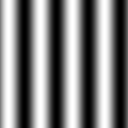
\includegraphics[scale=0.7]{mire1}\\
		mire1
	\end{center}
\end{figure}
\begin{figure}
	\begin{center}
		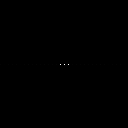
\includegraphics[scale=0.7]{mire1_FFT}\\
		FFT mire1
	\end{center}
\end{figure}
\begin{figure}
	\begin{center}
		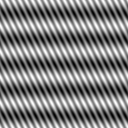
\includegraphics[scale=0.7]{mire3}\\
		mire3
	\end{center}
\end{figure}
\begin{figure}
	\begin{center}
		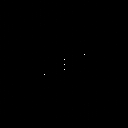
\includegraphics[scale=0.7]{mire3_FFT}\\
		FFT mire3
	\end{center}
\end{figure}
\begin{figure}
	\begin{center}
		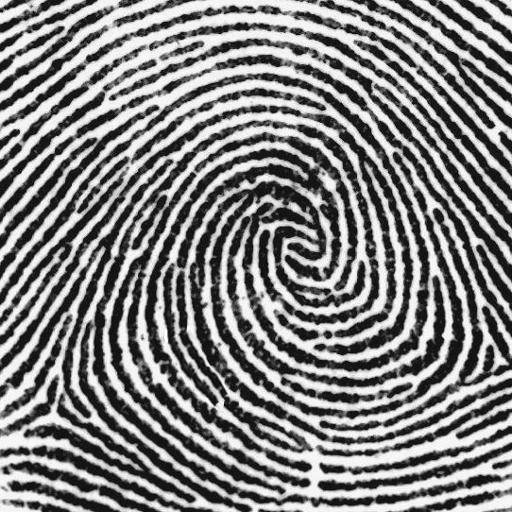
\includegraphics[scale=0.4]{fingerprint}\\
		fingerprint
	\end{center}
\end{figure}
\begin{figure}
	\begin{center}
		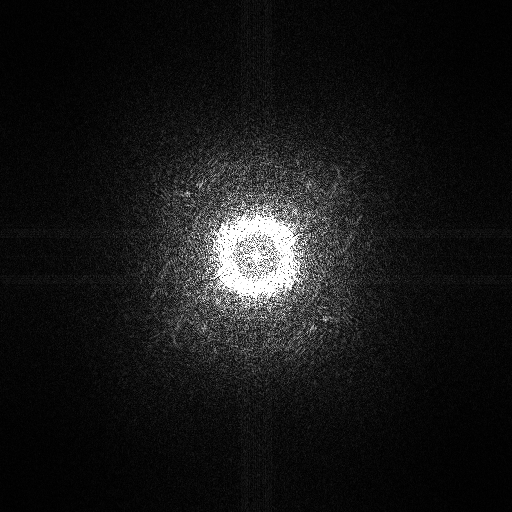
\includegraphics[scale=0.4]{fingerprint_FFT}\\
		FFT fingerprint
	\end{center}
\end{figure}
\begin{figure}
	\begin{center}
		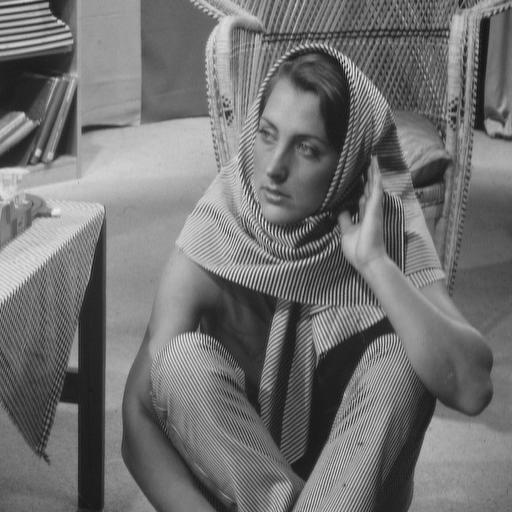
\includegraphics[scale=0.4]{barbara_512}\\
		barbara
	\end{center}
\end{figure}
\begin{figure}
	\begin{center}
		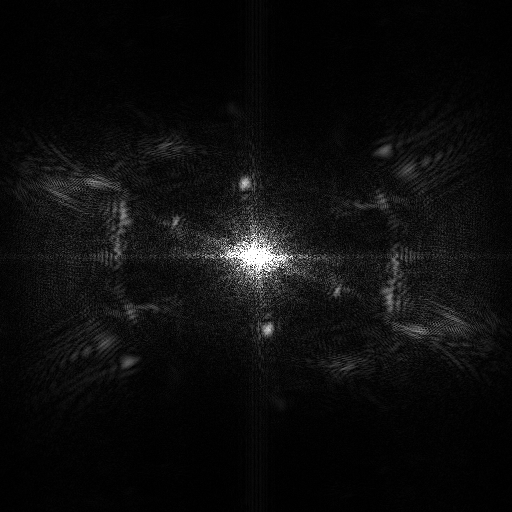
\includegraphics[scale=0.4]{barbara_FFT}\\
		FFT barbara
	\end{center}
\end{figure}
Pour la compression, il y a 2 méthodes. Soit on décide d'enlever toutes les hautes fréquences. On a juste à sélectionner la partie centrale de l'image et enlever tout le reste, notre oeil étant sensible aux basses fréquences. Ou d'enlever toutes les images en dessous d'un seuil fixé. Ainsi dans le cas des fréquences, la compression finie par montrer visuellement les différentes ondes (cf tigre compresse) alors que la compression par seuil va appliquer un effet de grain (cf tigre compresse seuil). Parfois, la compression peut donner des résultats surprenants, en enlevant par exemple les rayures de l'image de barbara. En effet, comme les fréquences décrivant ces rayures se trouvent à l'extérieure de l'image, la sélection par fréquence supprime les rayures de barbara.
\begin{figure}
	\begin{center}
		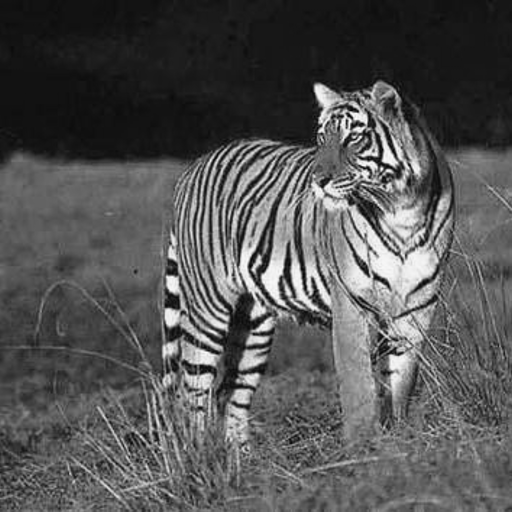
\includegraphics[scale=0.4]{tigre_512}\\
		tigre
	\end{center}
\end{figure}
\begin{figure}
	\begin{center}
		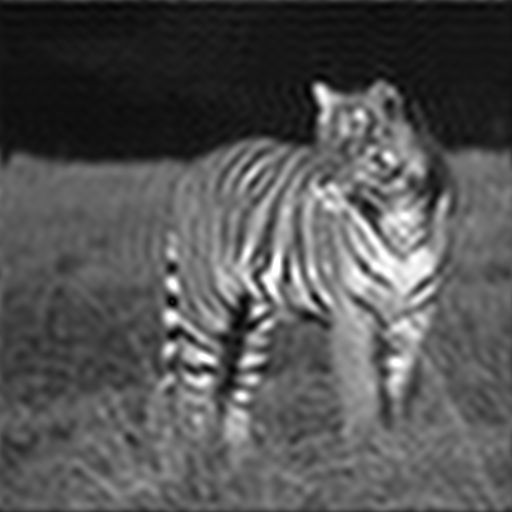
\includegraphics[scale=0.4]{tigre_compresse}\\
		Compression par fréquences
	\end{center}
\end{figure}
\begin{figure}
	\begin{center}
		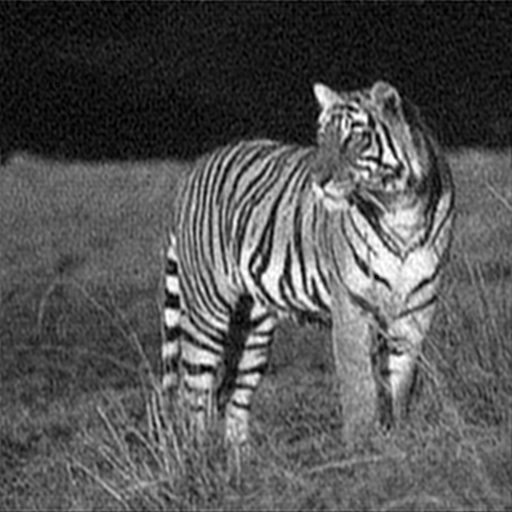
\includegraphics[scale=0.4]{tigre_compresse_seuil}\\
		Compression par seuil
	\end{center}
\end{figure}
\begin{figure}
	\begin{center}
		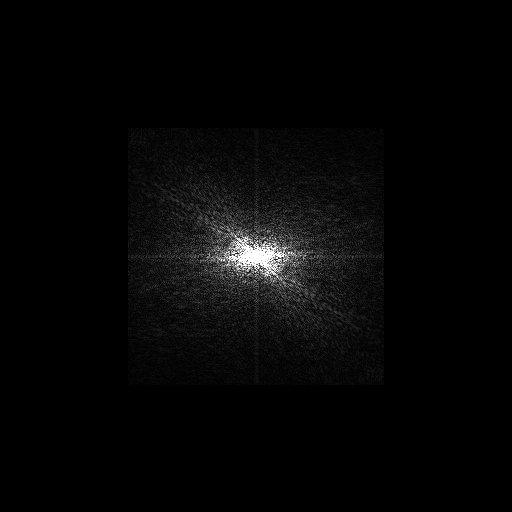
\includegraphics[scale=0.4]{lena_compresse}\\
		Compression par fréquences
	\end{center}
\end{figure}
\begin{figure}
	\begin{center}
		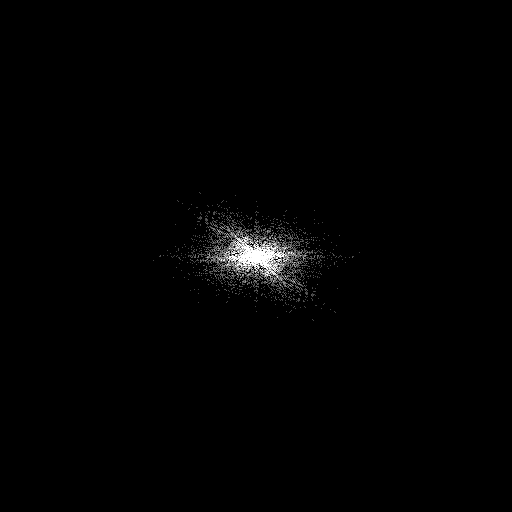
\includegraphics[scale=0.4]{lena_compresse_seuil}\\
		Compression par seuil
	\end{center}
\end{figure}
\begin{figure}
	\begin{center}
		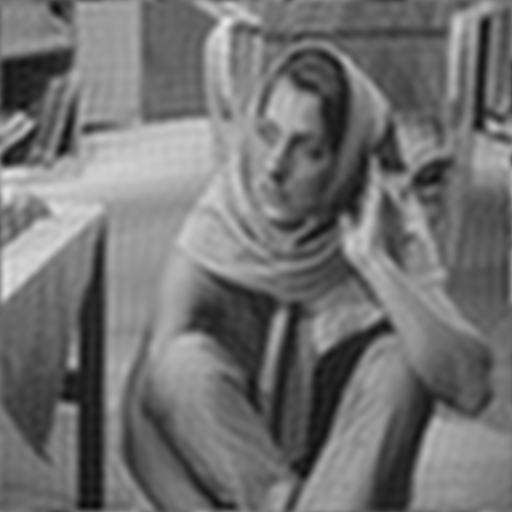
\includegraphics[scale=0.4]{barbara_compresse}\\
		Barbara compressée
	\end{center}
\end{figure}
\section{Conclusion}
Dans ce tp, on peut voir qu'il est parfois plus rapide de changer la forme des données pour travailler dessus (multiplication de polynomes ou la compression d'images ne sont que 2 exemples). La transformation prend du temps, mais ce temps est gagné par la suite avec des traitements rendus plus facile.
De plus, on remarque donc que la transformée de Fourier est très présente dès qu'il y a un traitement sur un signal à réaliser. Ici, nous n'avons vu qu'une toute petite partie de ses applications.

\end{document}

